\providecommand{\main}{../..}
\documentclass[\main/notes.tex]{subfiles}

\begin{document}
	\setcounter{chapter}{7}
	\chapter{Management Information and Decision Support Systems}
	\chaptermark{MIS and DSS}
		\section{Decision-Making and Problem-Solving}
			\begin{definition}{Decision-Making Phase}
				The first part of problem-solving, including three stages: intelligence, design, and choice.
			\end{definition}
			\begin{definition}{Problem-Solving}
				A process that goes beyond decision-making to include the implementation and monitoring stages.
			\end{definition}
			\begin{sidenote}{Decision-Making and Problem-Solving}
				\begin{minipage}{0.39\textwidth}
					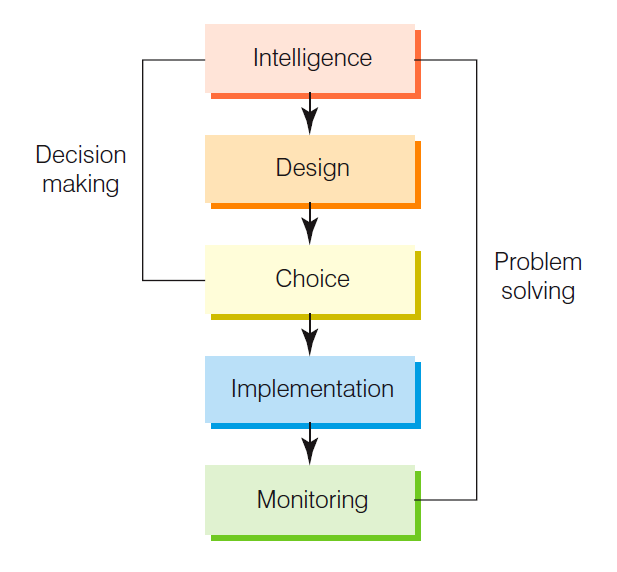
\includegraphics[width=0.9\linewidth]{chapter08/decision_making.png}
				\end{minipage}
				\begin{minipage}{0.6\textwidth}
					\begin{description}[]
						\item[Intelligence Stage] The first stage of decision-making, in which problems or opportunities are identified and defined.
						\item[Design Stage] The second stage of decision-making, in which alternative solutions to the problem are defined.
						\item[Choice Stage] The third stage of decision-making, which requires selecting a course of action.
						\item[Implementation Stage] A stage of problem-solving, in which a solution is put into effect.
						\item[Monitoring Stage] The final stage of the problem-solving process, in which decision-makers evaluate the implementation.
					\end{description}
				\end{minipage}
			\end{sidenote}
			\subsection{Programmed vs Non-Programmed Decisions}
				\begin{definition}{Programmed Decision}
					A decision made using a rule, procedure, or quantitative method.

					East to computerise using traditional information systems. They are structured, and deal with routine, well-defined decisions.
				\end{definition}
				\begin{definition}{Non-programmed Decision}
					A decision that deals with unusual or exceptional situations that can be difficult to quantify.
				\end{definition}
			\subsection{Optimisation, Satisficing, and Heuristic Approaches}
				\begin{definition}{Optimisation Model}
					A model that finds the best solution. These models use problem constraints.
				\end{definition}
				\begin{definition}{Satisficing Model}
					A model that will find a good, but not necessarily the best, problem solution.

					Usually used because modelling the problem properly to get an optimal decision would be too difficult, complex, or costly.

					Satisficing does not look at all possible solutions, but only those likely to give good results.
				\end{definition}
				\begin{definition}{Heuristics}
					Often referred to as \concept{rules of thumb}. Commonly accepted guidelines of procedures that usually find a good solution.
				\end{definition}
			\subsection{Sense and Respond}
				\begin{definition}{Sense and Respond (SaR)}
					Determining problems or opportunities (\concept{sense}), and developing systems to solve the problems or take advantage of the opportunities (\concept{respond}).

					Requires nimble organisations that replace traditional lines of authority with those that are flexible and dynamic.
				\end{definition}
			\subsection{Big Data}
				\begin{definition}{Big Data}
					Where the data that a company collects is so huge that it is difficult to process using traditional database technology.
				\end{definition}
	\vbox{\rulechapterend}
\end{document}